\documentclass{article}
\usepackage[english]{babel}
\usepackage[margin=1in,rmargin=1in,includefoot]{geometry} 
\usepackage{blindtext}
\usepackage{everysel}
\usepackage{fancyhdr} 
\usepackage{graphicx} 
\usepackage{float}
\usepackage{physics}
\usepackage{textcomp}
\usepackage{algorithm}
\usepackage{verbatim}
\usepackage[noend]{algpseudocode}
\usepackage[none]{hyphenat} 
\usepackage{amsfonts} 
\usepackage{subcaption}
\usepackage{amsmath} 
\usepackage{mathtools}
\usepackage{indentfirst}
\usepackage{lipsum}
\usepackage{tgcursor}
\usepackage{IEEEtrantools}
\usepackage{cases}
\usepackage{xcolor}
\usepackage{hyperref}

%\usepackage{CormorantGaramond}
\usefont{T1}{garamondMath}{m}{n}

%\usepackage[nf]{coelacanth}
%\let\oldnormalfont\normalfont
%\def\normalfont{\oldnormalfont\mdseries}

%\usepackage{TheanoOldStyle}

\usepackage[T1]{fontenc}
\usepackage[utf8]{inputenc}
\usepackage{ragged2e}


\pagestyle{fancy}
\fancyhead{} 
\fancyfoot{} 
\fancyhead[L]{\slshape \MakeUppercase{NLDC Assignment I}}
\fancyhead[R]{\slshape Anwesh Bhattacharya}
\fancyfoot[C]{\thepage} 

\EverySelectfont{%
\fontdimen2\font=0.4em% interword space
\fontdimen3\font=0.2em% interword stretch
\fontdimen4\font=0.1em% interword shrink
\fontdimen7\font=0.1em% extra space
\hyphenchar\font=`\-% to allow hyphenation
}
\renewcommand{\baselinestretch}{1.5}

\newcommand\textcite[2]{$\text{#1}^{\cite{#2}}$}
\newcommand\customfont[1]{{\usefont{T1}{garamond}{m}{n} #1 }}

\setlength{\parskip}{1em}

\hypersetup{
    colorlinks=true,
    linkcolor=blue,
    filecolor=magenta,      
    urlcolor=cyan,
    pdftitle={Sharelatex Example},
}
\urlstyle{same}
\hypersetup{
    pdftitle={Non-Linear Dynamics and Chaos : Assignment I},
    pdfauthor={Anwesh Bhattacharya},
    pdfsubject={Quantum Mechanic},
    bookmarksnumbered=true,     
    bookmarksopen=true,         
    bookmarksopenlevel=1,       
    colorlinks=true,            
    pdfstartview=Fit,           
    pdfpagemode=UseOutlines,    % this is the option you were looking for
}

\begin{document}

\title{\textbf{Canonical Transformations}}
\author{Anwesh Bhattacharya}
\maketitle
\hrule


\section{Action-Angle Variables}

\justify
The transformation from the action-angle variables to the usual co-ordinates is as follows -
\begin{align*} 
q &= \sqrt{\frac{2I}{m\omega}}\sin{\theta} \tag{7.1}\label{eq:7.1}
 \\
p &= \sqrt{2Im\omega} \cos(\theta) \tag{7.2}\label{eq:7.2}
\end{align*}

\justify
This can be inverted to obtain the canonical transformation -
\begin{align*} 
\theta &= \tan^{-1}{\left(\frac{m\omega q}{p}\right)}  \tag{7.3}\label{eq:7.3}\\
I &= \frac{p^2}{2m\omega} + \frac{m\omega q^2}{2} \tag{7.4}\label{eq:7.4}
\end{align*}

\justify
For the $F_1$ generating function, the following condition must be satisfied -
\begin{align*} 
\pdv{F_1(q,\theta)}{q} &= p = qm\omega \cot{\theta} \\
F_1 &= \int qm\omega \cot{\theta} dq \\
F_1 &= \frac{q^2 m\omega}{2}\cot{\theta} + h(\theta) \tag{7.5}\label{eq:7.5}
\end{align*}

\justify
$F_1$ is variable upto a function of $\theta$. Using the second equation of the generating function -
\begin{align*} 
\pdv{F_1(q,\theta)}{\theta} &= -I \\
-\frac{q^2 m\omega}{2}\csc^2{\theta} + h'(\theta)&= -I
\end{align*}

\justify
But from \eqref{eq:7.1}, we have $\displaystyle{I = \frac{q^2 m\omega}{2}\csc^2{\theta}}$, and thus $h'(\theta) = 0$. Since constants do not play a role in the generating function, we have the result -
$$\displaystyle{
F_1 = \frac{q^2 m\omega}{2} \cot{\theta}
}$$

\section{A Particular Generating Function}
\justify
The generating function $\displaystyle{F_1 = cq^2\cot{Q}}$ gives us the relations -
\begin{align*} 
p &= \pdv{F_1}{q} = 2cq\cot{Q} \tag{8.1}\label{eq:8.1} \\
P &= -\pdv{F_1}{Q} = cq^2\csc^2{Q} \implies q^2 = \frac{P}{c}\sin^2{Q} \tag{8.2}\label{eq:8.2} 
\end{align*}

\justify
Equation \eqref{eq:8.2} does not describe the canonical transformation entirely as it depends on $Q$. The transformation is correctly described as -
\begin{align*} 
Q &= \tan^{-1}{\left(\frac{2cq}{p}\right)}  \tag{8.3}\label{eq:8.3}\\
P &= \frac{p^2 + 4c^2q^2}{4c} \tag{8.4}\label{eq:8.4}
\end{align*}

\justify
Equation \eqref{eq:8.4} was obtained using \eqref{eq:8.3}, the pythagorean theorem and substituting into \eqref{eq:8.2}. Substituting these transformation equations into the hamiltonian $\displaystyle{H(q,p) = \frac{p^2}{2m} + \frac{m\omega^2 q^2}{2}}$, we get -
\begin{align*} 
K(Q,P) &= \frac{4c^2q^2}{2m}\cot^2{Q} + \frac{Pm\omega^2}{2c}\sin^2{Q}\\
&= \left(\frac{4c^2}{2m}\cot^2{Q} \times \frac{P}{c}\sin^2{Q}\right) + \frac{Pm\omega^2}{2c}\sin^2{Q} \\
&= \frac{2Pc}{m}\cos^2{Q} + \frac{Pm\omega^2}{2c}\sin^2{Q} \tag{8.5}\label{eq:8.5}
\end{align*}

\justify
Under this canonical transformation, the Hamilton's equations from \eqref{eq:8.5} are -
\begin{align*} 
\dot{P} &= -\pdv{K}{Q} = \frac{4Pc}{m}\sin{Q}\cos{Q} - \frac{Pm\omega^2}{c}\sin{Q}\cos{Q} \tag{8.6}\label{eq:8.6} \\
\dot{Q} &= \pdv{K}{P} = \frac{2c}{m}\cos^2{Q} + \frac{m\omega^2}{2c}\sin^2{Q} \tag{8.7}\label{eq:8.7}
\end{align*}

\justify
Observing that $\displaystyle{\dot{Q} = \frac{K}{P}}$, where $K$ is the value of the Hamiltonian at the initial condition $(Q_0, P_0)$, the equations of motions simplify to -
\begin{align*} 
\dot{P} &= \frac{P\sin{2Q}}{2}\left(\frac{4c}{m} - \frac{m\omega^2}{c}\right) \tag{8.7}\label{eq:8.7} \\
\dot{Q} &= \frac{K}{P} \tag{8.8}\label{eq:8.8}
\end{align*}

\justify
The above two equations is a system of differential equations in (Q,P) and is highly non-linear. However, a simplification can be observed by setting $\dot{P} = 0$ which gives $\displaystyle{c=\frac{m\omega}{2}}$. For this particular value of the constant $c$, the new variables reduce to the action-angle variables.

\subsection{Solving the Systems in the Old and New Variables}

\justify
%
In the old variables, the solution is trivial -
\begin{align*}
q = A\cos{(\omega t + \phi)} + B\sin{(\omega t + \phi)} \tag{8.9}\label{eq:8.9}\\
p = m\omega\left[B\cos{(\omega t + \phi)} - A\sin{(\omega t + \phi)}\right] \tag{8.10}\label{eq:8.10}
\end{align*}

\justify
The values of A, B are obtained from the initial conditions $(q_0, p_0)$. For the purposes of demonstration, let us set $m=1$ and $\omega=2$. In the old variables, the phase plot is as follows for $(q_0, p_0) = (0,1)$ -

\begin{figure}[!htb]
    \centering
    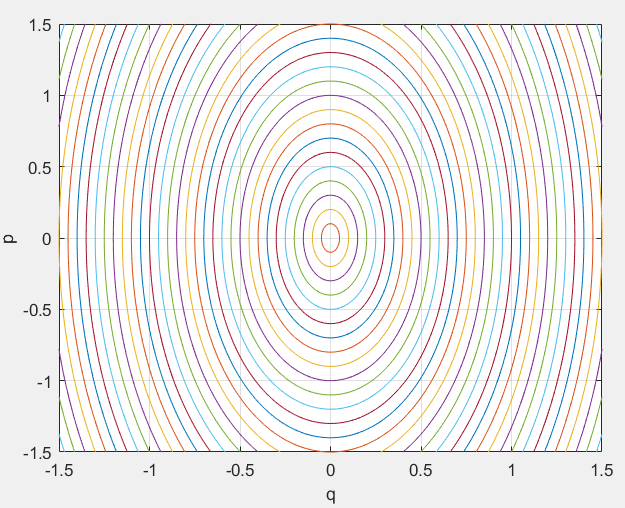
\includegraphics[width=3.5in,height=3.5in,keepaspectratio]{HarmonicPhasePotrait.PNG}
    \label{fig:oldHarmonic}
    \caption{Phase potrait of harmonic oscillator}
\end{figure}

\justify
According to the equations \eqref{eq:8.3} and \eqref{eq:8.4}, the initial conditions under the canonical transformation are $\displaystyle{(Q_0, P_0) = (0,\frac{1}{4c})}$. The value of $c$ such that this transformation degeneratoes to the action-angle variables is $\displaystyle{c=\frac{m\omega}{2} = 1}$. The initial value of the Hamiltonian is $\displaystyle{H = K = \eval{\frac{p^2}{2m} + \frac{m\omega^2q^2}{2}}_{(0,1)} = \frac{1}{2}}$. The range of the Q-axis is $[0,2\pi]$. 
\begin{figure}[!htb]
    \centering
    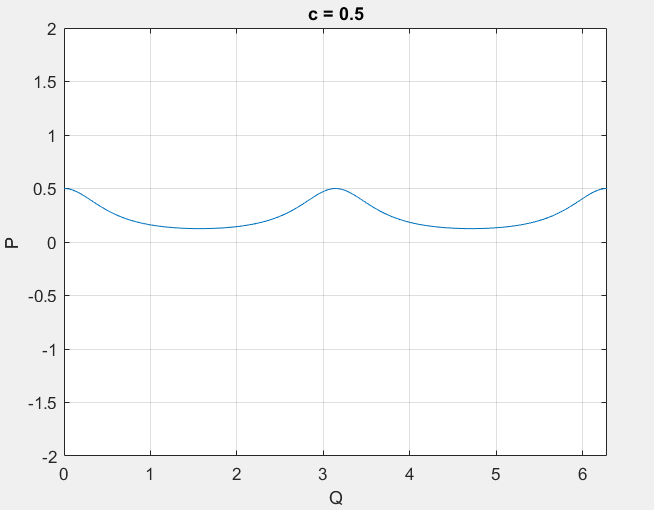
\includegraphics[width=3.5in,height=3.5in,keepaspectratio]{C0p5.PNG}
    \label{fig:C0p5}
    \caption{c = 0.5}
\end{figure}

\justify
The next plot is for $c=1$. This is expected to boil down to the action-angle transformation (\textit{and it does!})
\begin{figure}[!htb]
    \centering
    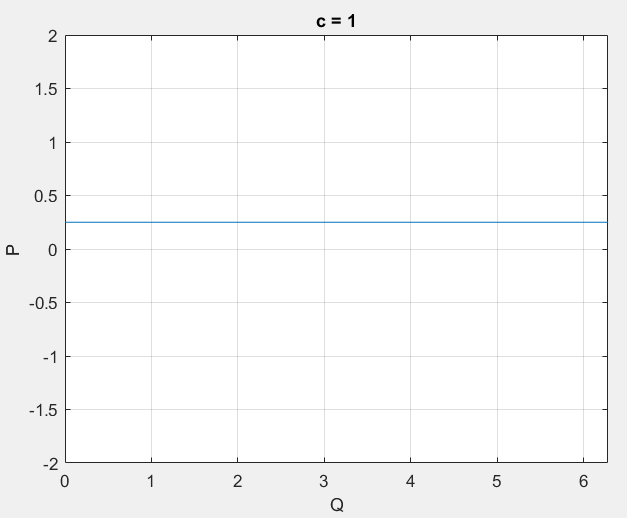
\includegraphics[width=3.5in,height=3.5in,keepaspectratio]{C1.PNG}
    \label{fig:C1}
    \caption{c = 1.0}
\end{figure}
\justify
The last figure is for $c = 2$ -
\begin{figure}[!htb]
    \centering
    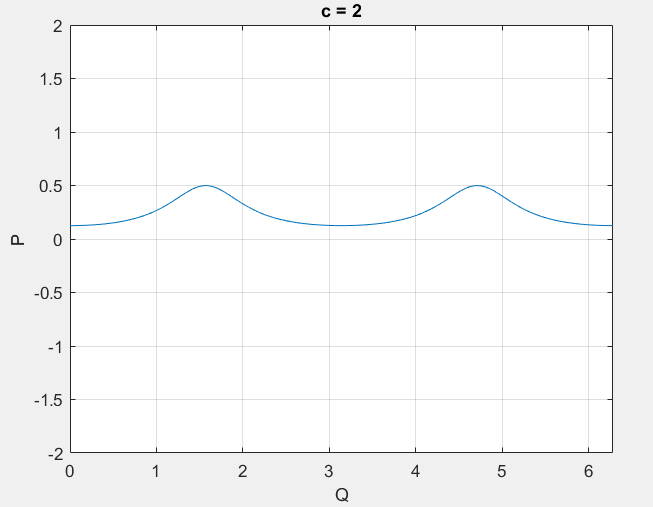
\includegraphics[width=3.5in,height=3.5in,keepaspectratio]{C2.PNG}
    \label{fig:C2}
    \caption{c = 2.0}
\end{figure}
\justify
It is also interesting to observe the phase potraits for various initial conditions $(q_0, p_0) \to (Q_0, P_0)$, for particular values of c. In the case of $c=\frac{1}{2}$, it will be a bunch of horizontal lines at various heights from the Q-axis. The following plot is the phase potrait for $c=0.9$. 

\begin{figure}[!htb]
    \centering
    \includegraphics[width=4.0in,height=4.0in,keepaspectratio]{PotraitC0p9.PNG}
    \label{fig:C0p9}
    \caption{Phase potrait for C=0.9}
\end{figure}

\justify
Finally, the following is the phase potrait for $c=3.0$ (\textit{next page})
\begin{figure}[!htb]
    \centering
    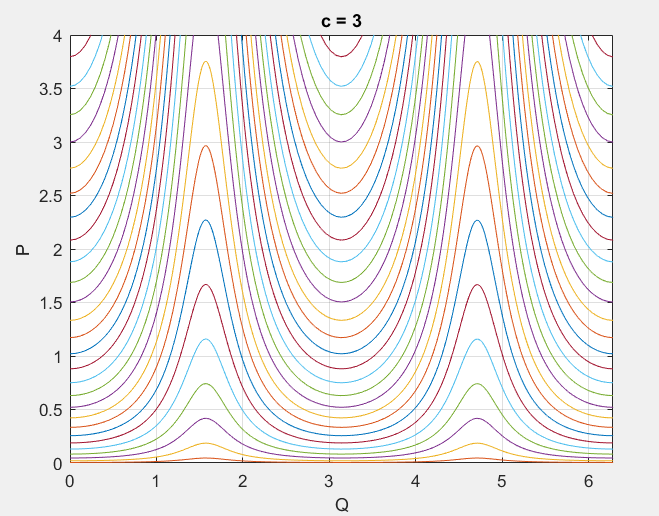
\includegraphics[width=4.0in,height=4.0in,keepaspectratio]{PotraitC3.PNG}
    \label{fig:C0p9}
    \caption{Phase potrait for C=3.0}
\end{figure}

\justify

It is easily noticeable the difference in the contours this image and the previous one. One is for $c < 2$ and the other is $c > 2$.


\end{document}
